\documentclass[preprint,12pt,aps,pra,showkeys,amsmath,amssymb,superscriptaddress,floatfix]{revtex4-2}
\usepackage[T1]{fontenc}
\usepackage[utf8]{inputenc}
\usepackage{amsmath,amssymb,amsthm,mathtools,mathrsfs}
\usepackage{microtype,booktabs,enumitem}
\usepackage{xcolor,tikz,etoolbox}
\usepackage[skins,breakable]{tcolorbox}
\usepackage{needspace}
% Keep diagram geometry independent of REVTeX preprint body spacing.
\AtBeginEnvironment{tikzpicture}{\linespread{1}\selectfont}
\usetikzlibrary{arrows.meta,positioning,calc,fit,decorations.pathreplacing}
\usepackage{graphicx}
\usepackage{hyperref}

\definecolor{MMBlue}{RGB}{0,82,155}
\definecolor{MMOrange}{RGB}{200,80,0}
\tikzset{
 mmnode/.style={draw=MMBlue,rounded corners=2pt,fill=MMBlue!4,align=left,execute at begin node={\raggedright},text width=5cm,font=\fontsize{10}{12}\selectfont,inner sep=6pt},
 mmimport/.style={mmnode,draw=black!65,fill=black!4},
 mmcandidate/.style={mmnode,draw=MMOrange,dashed,fill=MMOrange!5},
 mmrejected/.style={mmnode,draw=black,densely dotted,fill=black!8},
 mmproof/.style={->,thick,MMBlue},
 mmflow/.style={->,semithick,black!70},
 mmrepair/.style={->,dashed,thick,MMOrange},
 mmcandidatearrow/.style={->,dashed,semithick,MMOrange},
 mmnote/.style={font=\scriptsize,fill=white,inner sep=2pt,align=center}}

\usepackage[section]{placeins}
\setlength{\emergencystretch}{3em}
\setlist{itemsep=3pt,topsep=4pt}
\newtheorem{theorem}{Theorem}[section]
\newtheorem{proposition}[theorem]{Proposition}
\newtheorem{lemma}[theorem]{Lemma}
\newtheorem{corollary}[theorem]{Corollary}
\theoremstyle{definition}
\newtheorem{definition}[theorem]{Definition}
\newtheorem{example}[theorem]{Example}
\theoremstyle{remark}
\newtheorem{remark}[theorem]{Remark}
% Avoid isolated statement headings and single-line paragraph fragments.
\BeforeBeginEnvironment{theorem}{\Needspace{6\baselineskip}}
\BeforeBeginEnvironment{definition}{\Needspace{5\baselineskip}}
\BeforeBeginEnvironment{proposition}{\Needspace{5\baselineskip}}
\BeforeBeginEnvironment{lemma}{\Needspace{5\baselineskip}}
\BeforeBeginEnvironment{corollary}{\Needspace{5\baselineskip}}
\clubpenalty=5000
\widowpenalty=5000
\newcommand{\R}{\mathbb R}\newcommand{\Z}{\mathbb Z}\newcommand{\N}{\mathbb N}
\newcommand{\Pa}{\operatorname{Pa}}\newcommand{\Desc}{\operatorname{Desc}}
\newcommand{\cl}{\operatorname{cl}}\newcommand{\cost}{\operatorname{cost}}
\newcommand{\status}{\operatorname{status}}
% Faculty cards: a visual rail groups the five faculties within one agent.
% The rail has no arrowhead and does not represent a proof dependency.
\newcommand{\mmfacultybadge}[1]{%
 \node[circle,draw=MMBlue,line width=1pt,fill=white,
 minimum size=7mm,inner sep=0pt,font=\sffamily\small\bfseries,text=MMBlue]
 at ([xshift=15pt,yshift=-15pt]frame.north west) {#1};}
\newcommand{\mmfacultyrail}{%
 \draw[MMBlue!80,line width=1pt]
 ([xshift=15pt,yshift=2pt]frame.north west)--
 ([xshift=15pt,yshift=-2pt]frame.south west);}
\newtcolorbox{mmfacultybox}[2]{enhanced,breakable,
 colback=MMBlue!4,colframe=MMBlue!4,boxrule=0pt,arc=3pt,
 left=39pt,right=9pt,top=4pt,bottom=4pt,
 before skip=2pt,after skip=2pt,
 fontupper=\small\linespread{1.1}\selectfont,
 overlay unbroken={\mmfacultyrail\mmfacultybadge{#1}},
 overlay first={\mmfacultyrail\mmfacultybadge{#1}},
 overlay middle={\mmfacultyrail},overlay last={\mmfacultyrail}}
\newcommand{\mmfaculty}[3]{%
 \begin{mmfacultybox}{#1}{#2}
 {\sffamily\bfseries\color{MMBlue}#2}\par\smallskip #3
 \end{mmfacultybox}}
\newcommand{\agent}[9]{%
 \Needspace{8\baselineskip}
 \subsubsection{#1}
 \noindent\textbf{Object.} #2\par
 \noindent\textbf{Role.} #3\par\smallskip
 \mmfaculty{E}{Ego}{#4}
 \mmfaculty{M}{Memory}{#5}
 \mmfaculty{I}{Intellect}{#6}
 \mmfaculty{S}{Sense}{#7}
 \mmfaculty{A}{Action}{#8}
 \smallskip\noindent #9\par}

\usepackage{longtable,array,calc}
\providecommand{\tightlist}{\setlength{\itemsep}{2pt}\setlength{\parskip}{0pt}}
\makeatletter
\def\frontmatter@abstract@produce{\par\addvspace{\frontmatter@preabstractspace}%
\begingroup\prep@absbox\unvbox\absbox\post@absbox\endgroup
\addvspace{\frontmatter@postabstractspace}}
\makeatother
\newcommand{\field}[2]{\par\smallskip\noindent\textbf{#1.} #2\par}
\setlength{\emergencystretch}{5em}
\AtBeginEnvironment{verbatim}{\small\linespread{1.0}\selectfont}


\hypersetup{colorlinks=true,linkcolor=MMBlue,urlcolor=MMBlue,pdfauthor={Dibakar Sigdel}}

\begin{document}

\title{Schur's Lemma and Scalar Endomorphisms\\[4pt]\large An End-to-End Meta-Math Walkthrough}

\author{Dibakar Sigdel}

\affiliation{Mindverse Computing LLC, Lynnwood, WA 98087, USA}

\date{October 2026}

\begin{abstract}

Equivariance turns kernel and image into invariant subspaces. Algebraic
closure then produces a scalar that makes an endomorphism singular,
forcing it to vanish after subtraction. The report presents the target
theorem, declared imports, a dependency graph, five-faculty node
contracts, a continuous proof, a worked example, and a hypothesis-repair
audit. It is an authored mathematical exposition, not a deployed-agent
transcript or a formal proof-assistant certificate.

\end{abstract}\maketitle\linespread{1.12}\selectfont

\noindent\textbf{RT-02 / Representation Theory and Lie Theory / Report v1}

\section{Target and import contract}

\begin{theorem}

Let \(V,W\) be nonzero irreducible representations of a group \(G\) over
a field \(k\). Every nonzero intertwiner \(T:V\to W\) is an isomorphism.
If \(k\) is algebraically closed and \(V\) is finite-dimensional, every
equivariant endomorphism of \(V\) is scalar. Consequently for
finite-dimensional irreducibles over such \(k\),
\(\dim_k\operatorname{Hom}_G(V,W)\) is one when \(V\cong W\) and zero
otherwise.

\end{theorem}

\subsection{Foundations and permitted imports}

Use kernels and images of linear maps, eigenvalue existence for a linear
operator on a nonzero finite-dimensional vector space over an
algebraically closed field, and linear dimension. The first assertion
does not require finite dimension or algebraic closure.

\clearpage\section{Node interaction workflow}

\begin{center}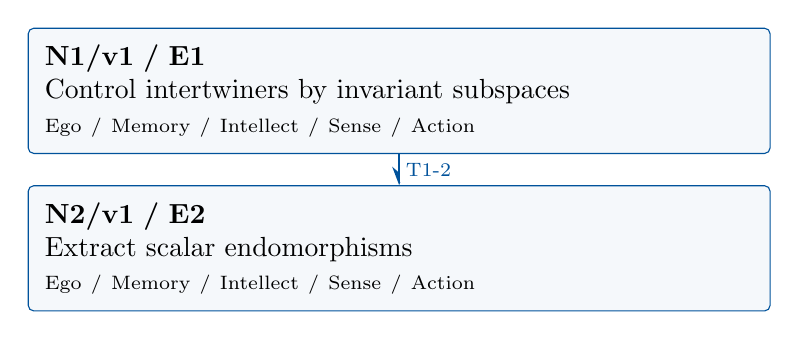
\begin{tikzpicture}[>=Stealth,x=1cm,y=1cm]

\node[mmnode,text width=9cm,minimum height=1.25cm] (N1) at (0,0.0) {\textbf{N1/v1 / E1}\\Control intertwiners by invariant subspaces\\{\scriptsize Ego / Memory / Intellect / Sense / Action}};

\node[mmnode,text width=9cm,minimum height=1.25cm] (N2) at (0,-2.0) {\textbf{N2/v1 / E2}\\Extract scalar endomorphisms\\{\scriptsize Ego / Memory / Intellect / Sense / Action}};

\draw[mmproof] (N1.south) -- node[mmnote,right] {T1-2} (N2.north);

\end{tikzpicture}\end{center}

Each box is one mathematical agent containing all five faculties. Blue
arrows carry the versioned exports listed below. The layout gives a
reading order; only drawn arrows assert dependencies. Diagnostic repair
is separate from the proof DAG.

\subsection{Versioned evidence-transfer ledger}

\begingroup\small\linespread{1.05}\selectfont

\Needspace{5\baselineskip}\field{T1-2: N1/E1/v1 to N2}{Every nonzero \(G\)-intertwiner \(T:V\to W\) is an equivariant
isomorphism.}

\field{Receiving activity}{N2.1}

\field{Compatibility}{E1/v1 and a finite-dimensional irreducible \(V\) over algebraically
closed \(k\). Check: Eigenvalue existence is precisely where algebraic
closure and finite dimension enter.}

\endgroup

\clearpage\section{Agent roles and five-faculty activities}\begingroup\small\linespread{1.05}\selectfont\setlist{itemsep=1pt,topsep=2pt}

\subsection{N1/v1: Control intertwiners by invariant subspaces}

\field{Object and role}{Apply irreducibility separately to the kernel and image. \textbf{Local
obligation:} Every nonzero \(G\)-intertwiner \(T:V\to W\) is an
equivariant isomorphism.}

\field{Inputs}{\(T\rho_V(g)=\rho_W(g)T\) for every \(g\), and irreducible \(V,W\).}

\mmfaculty{E}{Ego}{Publish E1/v1 only after establishing this obligation: Every nonzero
\(G\)-intertwiner \(T:V\to W\) is an equivariant isomorphism.}

\mmfaculty{M}{Memory}{\(T\rho_V(g)=\rho_W(g)T\) for every \(g\), and irreducible \(V,W\).
Retain the stated assumptions and import versions.}

\mmfaculty{I}{Intellect}{Apply irreducibility separately to the kernel and image.}

\mmfaculty{S}{Sense}{Nonzero \(T\) excludes the full kernel and zero image; check both
injectivity and surjectivity.}

\mmfaculty{A}{Action}{Carry out activities N1.1--N1.2 below, retaining each calculation and
construction as evidence.}

\smallskip\noindent\textbf{Numbered mathematical activities}

\begin{enumerate}[label=N1.\arabic*,leftmargin=3.4em]

\item If \(v\in\ker T\), then \(T\rho_V(g)v=\rho_W(g)Tv=0\), so the kernel is
invariant. The image is invariant because \(\rho_W(g)Tv=T\rho_V(g)v\).

\item Irreducibility gives \(\ker T=0\) or \(V\) and \(\operatorname{im}T=0\)
or \(W\). Nonzero \(T\) forces \(\ker T=0\) and image \(W\). Thus \(T\)
is a bijective linear map, and multiplying the intertwining equality by
its inverse shows that the inverse is also equivariant.

\end{enumerate}

\field{Export E1/v1}{Every nonzero \(G\)-intertwiner \(T:V\to W\) is an equivariant
isomorphism.}

\field{Acceptance gate}{Nonzero \(T\) excludes the full kernel and zero image; check both
injectivity and surjectivity.}

\field{Targeted repair}{If only injectivity has been shown, use irreducibility of the codomain
to establish surjectivity. Withhold this export and recheck its
descendants after a versioned correction.}

\clearpage

\subsection{N2/v1: Extract scalar endomorphisms}

\field{Object and role}{Subtract an eigenvalue, then apply the nonzero-isomorphism alternative.
\textbf{Local obligation:} \(\operatorname{End}_G(V)=k\,\mathrm{id}\)
and the stated Hom-space dimensions follow.}

\field{Inputs}{E1/v1 and a finite-dimensional irreducible \(V\) over algebraically
closed \(k\). Incoming proof exports: E1/v1 at N2.1.}

\mmfaculty{E}{Ego}{Publish E2/v1 only after establishing this obligation:
\(\operatorname{End}_G(V)=k\,\mathrm{id}\) and the stated Hom-space
dimensions follow.}

\mmfaculty{M}{Memory}{E1/v1 and a finite-dimensional irreducible \(V\) over algebraically
closed \(k\). Incoming proof exports: E1/v1 at N2.1. Retain the stated
assumptions and import versions.}

\mmfaculty{I}{Intellect}{Subtract an eigenvalue, then apply the nonzero-isomorphism alternative.}

\mmfaculty{S}{Sense}{Eigenvalue existence is precisely where algebraic closure and finite
dimension enter.}

\mmfaculty{A}{Action}{Carry out activities N2.1--N2.2 below, retaining each calculation and
construction as evidence.}

\smallskip\noindent\textbf{Numbered mathematical activities}

\begin{enumerate}[label=N2.\arabic*,leftmargin=3.4em]

\item For \(A\in\operatorname{End}_G(V)\) choose an eigenvalue
\(\lambda\in k\). The map \(A-\lambda I\) is equivariant and has a
nonzero kernel. E1 says it cannot be a nonzero map, because then it
would be invertible. Therefore \(A=\lambda I\).

\item If \(V\not\cong W\), E1 rules out every nonzero intertwiner. If
\(S:V\to W\) is a fixed isomorphism, every intertwiner \(T\) satisfies
\(S^{-1}T\in\operatorname{End}_G(V)\), so \(T=\lambda S\). Thus the
Hom-space is one-dimensional in the isomorphic case.

\end{enumerate}

\field{Export E2/v1}{\(\operatorname{End}_G(V)=k\,\mathrm{id}\) and the stated Hom-space
dimensions follow.}

\field{Acceptance gate}{Eigenvalue existence is precisely where algebraic closure and finite
dimension enter.}

\field{Targeted repair}{If a real irreducible endomorphism is declared scalar, check whether it
has a real eigenvalue; retain the algebraically closed field for this
conclusion. Withhold this export and recheck its descendants after a
versioned correction.}

\endgroup\clearpage\section{Continuous mathematical proof}\label{sec:proof}

\subsection{N1 --- Control intertwiners by invariant
subspaces}\label{n1-control-intertwiners-by-invariant-subspaces}

\begin{enumerate}
\def\labelenumi{\arabic{enumi}.}
\item
  \textbf{N1.1.} If \(v\in\ker T\), then \(T\rho_V(g)v=\rho_W(g)Tv=0\),
  so the kernel is invariant. The image is invariant because
  \(\rho_W(g)Tv=T\rho_V(g)v\).
\item
  \textbf{N1.2.} Irreducibility gives \(\ker T=0\) or \(V\) and
  \(\operatorname{im}T=0\) or \(W\). Nonzero \(T\) forces \(\ker T=0\)
  and image \(W\). Thus \(T\) is a bijective linear map, and multiplying
  the intertwining equality by its inverse shows that the inverse is
  also equivariant.
\end{enumerate}

\subsection{N2 --- Extract scalar
endomorphisms}\label{n2-extract-scalar-endomorphisms}

\begin{enumerate}
\def\labelenumi{\arabic{enumi}.}
\item
  \textbf{N2.1.} For \(A\in\operatorname{End}_G(V)\) choose an
  eigenvalue \(\lambda\in k\). The map \(A-\lambda I\) is equivariant
  and has a nonzero kernel. E1 says it cannot be a nonzero map, because
  then it would be invertible. Therefore \(A=\lambda I\).
\item
  \textbf{N2.2.} If \(V\not\cong W\), E1 rules out every nonzero
  intertwiner. If \(S:V\to W\) is a fixed isomorphism, every intertwiner
  \(T\) satisfies \(S^{-1}T\in\operatorname{End}_G(V)\), so
  \(T=\lambda S\). Thus the Hom-space is one-dimensional in the
  isomorphic case.
\end{enumerate}

\hfill$\square$

\section{Worked orchestration}

For the one-dimensional complex characters of \(C_3\), let a generator
act by \(\omega\) on \(V\) and by \(\omega^2\) on \(W\), where
\(\omega^3=1\) and \(\omega\ne1\). A linear map is multiplication by
\(a\), and equivariance gives \(a\omega=\omega^2a\), hence \(a=0\). Each
character's endomorphism algebra is \(\mathbb C\).

\subsection{Boundary and hypothesis audit}

Over \(\mathbb R\), let \(C_4\) act on \(\mathbb R^2\) by a rotation
\(J\) through \(90\) degrees. There is no invariant real line, so the
representation is irreducible. Yet \(J\) commutes with the action and is
not a real scalar matrix. The first part of Schur's lemma holds; the
scalar conclusion does not.

\section{Illustrative failure and repair}

The following is an authored diagnostic scenario. Changed assumptions
define a new contract; they do not retroactively prove the original
statement.

\subsection{Rejected argument, diagnosis, and correction}
\textbf{Rejected N2 export:} every endomorphism of a real irreducible
representation is scalar. \textbf{Sense witness:} the rotation \(J\).
\textbf{Diagnosis:} Memory imported an eigenvalue over a field where
none need exist. \textbf{Repair:} apply scalar Schur only over the
algebraically closed field in §1. The broader real conclusion is
replaced by the weaker statement that nonzero equivariant endomorphisms
are invertible. The complex theorem is unchanged.

\subsection{Publication and reuse}
The corrected export retains its explicit assumptions. A hypothetical
revision receives a new version, and each consuming activity is
rechecked; this scenario is not a recorded runtime event. \textbf{Next
direction:} Use the Hom-space dimension in RT-03 to convert an averaging
projection into character orthogonality.

\par\medskip\begingroup\small\linespread{1.0}\selectfont\noindent\textbf{Provenance.} This authored proof is complete relative to its declared imports. Reuse
each export with its assumptions, proof, and version. The original
Markdown remains available for comparison.
\par\endgroup

\par\smallskip\begingroup\small\linespread{1.0}\selectfont\noindent\textbf{Further reading.} \href{https://math.mit.edu/~etingof/reprbook.pdf}{Etingof and
collaborators, Introduction to Representation Theory}, sections on
representations, characters, and \(\mathfrak{sl}_2\);
\href{https://ocw.mit.edu/courses/18-745-lie-groups-and-lie-algebras-i-fall-2020/lists/lecture-notes/}{MIT
Lie Groups and Lie Algebras I lecture notes} for solvable Lie algebras.\par\endgroup

\end{document}
